% Options for packages loaded elsewhere
\PassOptionsToPackage{unicode}{hyperref}
\PassOptionsToPackage{hyphens}{url}
\PassOptionsToPackage{dvipsnames,svgnames,x11names}{xcolor}
%
\documentclass[
  10pt,
]{article}
\usepackage{amsmath,amssymb}
\usepackage{iftex}
\ifPDFTeX
  \usepackage[T1]{fontenc}
  \usepackage[utf8]{inputenc}
  \usepackage{textcomp} % provide euro and other symbols
\else % if luatex or xetex
  \usepackage{unicode-math} % this also loads fontspec
  \defaultfontfeatures{Scale=MatchLowercase}
  \defaultfontfeatures[\rmfamily]{Ligatures=TeX,Scale=1}
\fi
\usepackage{lmodern}
\ifPDFTeX\else
  % xetex/luatex font selection
  \setmainfont[]{DejaVu Serif}
  \setsansfont[]{DejaVu Sans}
  \setmonofont[]{DejaVu Sans Mono}
  \setmathfont[]{Latin Modern Math}
\fi
% Use upquote if available, for straight quotes in verbatim environments
\IfFileExists{upquote.sty}{\usepackage{upquote}}{}
\IfFileExists{microtype.sty}{% use microtype if available
  \usepackage[]{microtype}
  \UseMicrotypeSet[protrusion]{basicmath} % disable protrusion for tt fonts
}{}
\makeatletter
\@ifundefined{KOMAClassName}{% if non-KOMA class
  \IfFileExists{parskip.sty}{%
    \usepackage{parskip}
  }{% else
    \setlength{\parindent}{0pt}
    \setlength{\parskip}{6pt plus 2pt minus 1pt}}
}{% if KOMA class
  \KOMAoptions{parskip=half}}
\makeatother
\usepackage{xcolor}
\usepackage[margin=2.0cm]{geometry}
\usepackage{color}
\usepackage{fancyvrb}
\newcommand{\VerbBar}{|}
\newcommand{\VERB}{\Verb[commandchars=\\\{\}]}
\DefineVerbatimEnvironment{Highlighting}{Verbatim}{commandchars=\\\{\}}
% Add ',fontsize=\small' for more characters per line
\newenvironment{Shaded}{}{}
\newcommand{\AlertTok}[1]{\textcolor[rgb]{1.00,0.00,0.00}{\textbf{#1}}}
\newcommand{\AnnotationTok}[1]{\textcolor[rgb]{0.38,0.63,0.69}{\textbf{\textit{#1}}}}
\newcommand{\AttributeTok}[1]{\textcolor[rgb]{0.49,0.56,0.16}{#1}}
\newcommand{\BaseNTok}[1]{\textcolor[rgb]{0.25,0.63,0.44}{#1}}
\newcommand{\BuiltInTok}[1]{\textcolor[rgb]{0.00,0.50,0.00}{#1}}
\newcommand{\CharTok}[1]{\textcolor[rgb]{0.25,0.44,0.63}{#1}}
\newcommand{\CommentTok}[1]{\textcolor[rgb]{0.38,0.63,0.69}{\textit{#1}}}
\newcommand{\CommentVarTok}[1]{\textcolor[rgb]{0.38,0.63,0.69}{\textbf{\textit{#1}}}}
\newcommand{\ConstantTok}[1]{\textcolor[rgb]{0.53,0.00,0.00}{#1}}
\newcommand{\ControlFlowTok}[1]{\textcolor[rgb]{0.00,0.44,0.13}{\textbf{#1}}}
\newcommand{\DataTypeTok}[1]{\textcolor[rgb]{0.56,0.13,0.00}{#1}}
\newcommand{\DecValTok}[1]{\textcolor[rgb]{0.25,0.63,0.44}{#1}}
\newcommand{\DocumentationTok}[1]{\textcolor[rgb]{0.73,0.13,0.13}{\textit{#1}}}
\newcommand{\ErrorTok}[1]{\textcolor[rgb]{1.00,0.00,0.00}{\textbf{#1}}}
\newcommand{\ExtensionTok}[1]{#1}
\newcommand{\FloatTok}[1]{\textcolor[rgb]{0.25,0.63,0.44}{#1}}
\newcommand{\FunctionTok}[1]{\textcolor[rgb]{0.02,0.16,0.49}{#1}}
\newcommand{\ImportTok}[1]{\textcolor[rgb]{0.00,0.50,0.00}{\textbf{#1}}}
\newcommand{\InformationTok}[1]{\textcolor[rgb]{0.38,0.63,0.69}{\textbf{\textit{#1}}}}
\newcommand{\KeywordTok}[1]{\textcolor[rgb]{0.00,0.44,0.13}{\textbf{#1}}}
\newcommand{\NormalTok}[1]{#1}
\newcommand{\OperatorTok}[1]{\textcolor[rgb]{0.40,0.40,0.40}{#1}}
\newcommand{\OtherTok}[1]{\textcolor[rgb]{0.00,0.44,0.13}{#1}}
\newcommand{\PreprocessorTok}[1]{\textcolor[rgb]{0.74,0.48,0.00}{#1}}
\newcommand{\RegionMarkerTok}[1]{#1}
\newcommand{\SpecialCharTok}[1]{\textcolor[rgb]{0.25,0.44,0.63}{#1}}
\newcommand{\SpecialStringTok}[1]{\textcolor[rgb]{0.73,0.40,0.53}{#1}}
\newcommand{\StringTok}[1]{\textcolor[rgb]{0.25,0.44,0.63}{#1}}
\newcommand{\VariableTok}[1]{\textcolor[rgb]{0.10,0.09,0.49}{#1}}
\newcommand{\VerbatimStringTok}[1]{\textcolor[rgb]{0.25,0.44,0.63}{#1}}
\newcommand{\WarningTok}[1]{\textcolor[rgb]{0.38,0.63,0.69}{\textbf{\textit{#1}}}}
\usepackage{longtable,booktabs,array}
\usepackage{calc} % for calculating minipage widths
% Correct order of tables after \paragraph or \subparagraph
\usepackage{etoolbox}
\makeatletter
\patchcmd\longtable{\par}{\if@noskipsec\mbox{}\fi\par}{}{}
\makeatother
% Allow footnotes in longtable head/foot
\IfFileExists{footnotehyper.sty}{\usepackage{footnotehyper}}{\usepackage{footnote}}
\makesavenoteenv{longtable}
\usepackage{graphicx}
\makeatletter
\def\maxwidth{\ifdim\Gin@nat@width>\linewidth\linewidth\else\Gin@nat@width\fi}
\def\maxheight{\ifdim\Gin@nat@height>\textheight\textheight\else\Gin@nat@height\fi}
\makeatother
% Scale images if necessary, so that they will not overflow the page
% margins by default, and it is still possible to overwrite the defaults
% using explicit options in \includegraphics[width, height, ...]{}
\setkeys{Gin}{width=\maxwidth,height=\maxheight,keepaspectratio}
% Set default figure placement to htbp
\makeatletter
\def\fps@figure{htbp}
\makeatother
\setlength{\emergencystretch}{3em} % prevent overfull lines
\providecommand{\tightlist}{%
  \setlength{\itemsep}{0pt}\setlength{\parskip}{0pt}}
\setcounter{secnumdepth}{-\maxdimen} % remove section numbering
% doc_header.tex -- LaTeX preamble additions used by build_docs.sh for every
% Markdown -> LaTeX -> PDF conversion (supplements, README, submission files).
\usepackage{etoolbox}
% longtable may not be loaded by pandoc when a document has no table
\usepackage{longtable}
% bold vectors: \bm -> \symbf under unicode-math (XeLaTeX), bm package otherwise
\makeatletter
\@ifpackageloaded{unicode-math}{\providecommand{\bm}[1]{\symbf{#1}}}{\usepackage{bm}}
\makeatother
% smaller type in long tables so that wide audit tables fit the text width;
% inside a table a line break is allowed after an underscore of plain text
% (pandoc writes it as \_), so that long identifiers wrap inside their column
% rows are set a little apart, so that symbols with indices do not touch
\AtBeginEnvironment{longtable}{\footnotesize\renewcommand{\arraystretch}{1.45}%
  \let\sptunderscore\_\def\_{\sptunderscore\allowbreak}}
\setlength{\LTcapwidth}{\textwidth}
% allow line breaks after slashes and hyphens inside table cells
\usepackage{xurl}
% code blocks: break over-long lines instead of running into the margin.
% Plain ``` blocks are typeset by pandoc as {verbatim}, highlighted ones
% (```bash) as {Highlighting}; both are re-declared as breakable fancyvrb
% environments.  The continuation line is marked with a small hooked arrow.
\usepackage{fvextra}
\RecustomVerbatimEnvironment{verbatim}{Verbatim}{breaklines,breakanywhere,fontsize=\small}
\makeatletter
\@ifundefined{Highlighting}{}{%
  \RecustomVerbatimEnvironment{Highlighting}{Verbatim}{breaklines,breakanywhere,fontsize=\small,commandchars=\\\{\}}}
\makeatother
% inline code (pandoc writes it as \texttt{...}): never hyphenate -- an inserted
% hyphen could be read as part of a file name -- but allow a line break after
% an underscore, slash, comma, colon or equals sign, so that long paths and
% column lists wrap inside the text width and inside table columns.
% Inside a formula (e.g. the name of a notebook symbol in an equation) the same
% command must first leave math mode, which \text of amsmath does.
\ExplSyntaxOn
\tl_new:N \l__spt_code_tl
\cs_new_protected:Npn \__spt_texttt:n #1
  {
    \tl_set:Nn \l__spt_code_tl {#1}
    \regex_replace_all:nnN { ([\/\,\:\=]) } { \1 \c{allowbreak} } \l__spt_code_tl
    \regex_replace_all:nnN { \c{_} } { \c{_} \c{allowbreak} } \l__spt_code_tl
    \group_begin: \ttfamily \hyphenchar \font = -1 \scan_stop: \l__spt_code_tl \group_end:
  }
\RenewDocumentCommand \texttt { m }
  {
    \mode_if_math:TF { \text { \__spt_texttt:n {#1} } } { \__spt_texttt:n {#1} }
  }
\ExplSyntaxOff
% A figure is written in the Markdown source as an image paragraph followed by
% a caption paragraph ("**Figure S1.** ..."), so that the caption is also
% visible on GitHub.  An image that starts a paragraph is centered.
\usepackage{graphicx}% pandoc loads it only for documents that contain an image
\NewCommandCopy\sptincludegraphics\includegraphics
\RenewDocumentCommand\includegraphics{O{} m}{%
  \ifvmode\begin{center}\sptincludegraphics[#1]{#2}\end{center}%
  \else\sptincludegraphics[#1]{#2}\fi}
% keep figures where they are referenced
\usepackage{float}
\floatplacement{figure}{H}
% running header with the document title
\usepackage{fancyhdr}
\pagestyle{fancy}
\fancyhf{}
\fancyhead[L]{\small PROJECT spacetimes, Revision\_Deflation --- documentation and provenance}
\fancyhead[R]{\small\thepage}
\renewcommand{\headrulewidth}{0.4pt}
% 16x16 matrices: tighter columns so that a full matrix fits the text width
\setlength{\arraycolsep}{3.2pt}
% The documents of this project contain long tagged symbols, file paths and
% identifiers that cannot be hyphenated.  A paragraph is therefore allowed to
% have looser lines before TeX gives up and lets a line stick out of the margin.
\AtBeginDocument{\tolerance=2000 \emergencystretch=5em \hbadness=2000}
\ifLuaTeX
  \usepackage{selnolig}  % disable illegal ligatures
\fi
\IfFileExists{bookmark.sty}{\usepackage{bookmark}}{\usepackage{hyperref}}
\IfFileExists{xurl.sty}{\usepackage{xurl}}{} % add URL line breaks if available
\urlstyle{same}
\hypersetup{
  pdftitle={RS2 --- The hypothesis that the singlet superfluid is the Higgs field, on the deflating 4+4 and 7+1 spacetimes},
  pdfauthor={Prepared for Patrick Lee Nash, Ph.D.},
  colorlinks=true,
  linkcolor={blue},
  filecolor={Maroon},
  citecolor={blue},
  urlcolor={blue},
  pdfcreator={LaTeX via pandoc}}

\title{RS2 --- The hypothesis that the singlet superfluid is the Higgs
field, on the deflating 4+4 and 7+1 spacetimes}
\usepackage{etoolbox}
\makeatletter
\providecommand{\subtitle}[1]{% add subtitle to \maketitle
  \apptocmd{\@title}{\par {\large #1 \par}}{}{}
}
\makeatother
\subtitle{PROJECT spacetimes, Revision\_Deflation. Supplement to both
manuscripts of the revision}
\author{Prepared for Patrick Lee Nash, Ph.D.}
\date{November 13, 2026}

\begin{document}
\maketitle

\hypertarget{purpose-and-result}{%
\section{0. Purpose and result}\label{purpose-and-result}}

The author's task states the hypothesis, called \textbf{H2} in the main
project, that the superfluid singlet state --- the condensate of the
fermion pair along the hidden axis \(x0\) --- \emph{is the Higgs field}.
The supplement S2 of the main project tests the hypothesis against seven
conditions, C1 to C7, that a Higgs field must meet, on the two flat
spacetimes. This supplement repeats the test on the two spacetimes of
the revision, in which \(x5\), \(x6\), \(x7\) deflate. It is written for
a reader who has S2 at hand; the conditions are restated in Sec. 1.

\textbf{Result.} The deflation changes the standing of the hypothesis in
three ways.

\begin{enumerate}
\def\labelenumi{\arabic{enumi}.}
\tightlist
\item
  \emph{What supported the hypothesis on the flat 7+1 spacetime is
  weakened.} There, the condensate breaks the rotation group \(SO(4)\)
  of the four extra space axes to \(SO(3)\), the pattern of the Higgs
  vacuum, and the \(SO(4)\) is a symmetry of the spacetime. On the
  deflating 7+1 spacetime the rotations that mix \(x0\) with a deflating
  coordinate are no longer symmetries of the spacetime. The internal
  symmetry survives, exactly, as a symmetry of the fields that do not
  depend on the extra coordinates; but it is now a \emph{hidden}
  symmetry, as it was all along on 4+4 (Sec. 3).
\item
  \emph{The condensate in the vacuum} (condition C2), open on flat
  spacetime because it needs a coupling \(\alpha_{VS}\) of about 2 or
  more, is reached by the deflation at a definite time --- but outside
  the range in which the model can be trusted (Sec. 4).
\item
  \emph{A new and severe condition appears.} If the Higgs field is the
  pair condensate, the electroweak scale depends on the coupling
  \(\alpha_{VS}\), and \(\alpha_{VS}\) grows with the deflation. The
  masses of the ordinary fermions would then change with time, and
  atomic clocks exclude this unless the present rate of deflation is
  below about \(10^{-6}\) of the Hubble constant (Sec. 5). \textbf{The
  hypothesis H2 and a deflation that is of any consequence today exclude
  each other.}
\end{enumerate}

\hypertarget{how-to-reproduce}{%
\subsection{0.1 How to reproduce}\label{how-to-reproduce}}

\begin{Shaded}
\begin{Highlighting}[]
\BuiltInTok{cd} \StringTok{"/Users/nsh/Developer/github/spacetimes/Revision\_Deflation"}
\ExtensionTok{cargo}\NormalTok{ build }\AttributeTok{{-}{-}release} \AttributeTok{{-}{-}manifest{-}path}\NormalTok{ code/deflation{-}rs/Cargo.toml}
\ExtensionTok{./code/deflation{-}rs/target/release/deflation}\NormalTok{ symmetry    }\CommentTok{\# Secs. 2 and 3}
\ExtensionTok{./code/deflation{-}rs/target/release/deflation}\NormalTok{ cosmology   }\CommentTok{\# Sec. 5 (check def{-}C6)}
\ExtensionTok{python3}\NormalTok{ code/scripts/make\_figures.py isometries bounds}
\ExtensionTok{python3}\NormalTok{ code/scripts/write\_doc\_tables.py}
\ExtensionTok{python3}\NormalTok{ code/scripts/assemble\_docs.py docs\_src/RS2\_higgs\_hypothesis\_deflating.src.md}
\FunctionTok{bash}\NormalTok{ code/scripts/build\_docs.sh supplement/RS2\_higgs\_hypothesis\_deflating.md}
\end{Highlighting}
\end{Shaded}

\begin{center}\rule{0.5\linewidth}{0.5pt}\end{center}

\hypertarget{the-hypothesis-and-the-conditions}{%
\section{1. The hypothesis and the
conditions}\label{the-hypothesis-and-the-conditions}}

In the Standard Model the Higgs field is a doublet of the weak-isospin
group with a vacuum value \(v_{\rm EW}=246.22\) GeV, which breaks the
electroweak symmetry, gives the \(W\) and \(Z\) bosons and the quarks
and charged leptons their masses, and leaves one scalar particle of 125
GeV. Its four real components form a vector of a group \(SO(4)\), which
the vacuum value breaks to \(SO(3)\). S2 derives from this the
conditions that a condensate must satisfy in order to \emph{be} the
Higgs field:

\begin{longtable}[]{@{}
  >{\raggedright\arraybackslash}p{(\columnwidth - 2\tabcolsep) * \real{0.0968}}
  >{\raggedright\arraybackslash}p{(\columnwidth - 2\tabcolsep) * \real{0.9032}}@{}}
\toprule\noalign{}
\begin{minipage}[b]{\linewidth}\raggedright
\end{minipage} & \begin{minipage}[b]{\linewidth}\raggedright
Condition
\end{minipage} \\
\midrule\noalign{}
\endhead
\bottomrule\noalign{}
\endlastfoot
C1 & it is a scalar under the Lorentz group of ordinary spacetime \\
C2 & it is non-zero in empty space \\
C3 & it is a doublet of the weak-isospin group with a neutral
component \\
C4 & it breaks \(SO(4)\) to \(SO(3)\) \\
C5 & its scale is 246 GeV, with a scalar particle of 125 GeV with the
observed couplings \\
C6 & its couplings give the quarks and leptons their masses \\
C7 & no further light or charged particles accompany it that would have
been seen \\
\end{longtable}

\textbf{Two statements that must be kept apart.}

\begin{itemize}
\tightlist
\item
  \textbf{H2} is the author's hypothesis: the \emph{pair condensate} is
  the Higgs field. The electroweak scale is then the scale of the
  condensate.
\item
  \textbf{HV} is a different assumption, used in one place of the
  supplement RS3: the vacuum value of the \emph{Vorton-Scalar} sets the
  electroweak scale. S2 already notes that the Vorton-Scalar is a
  singlet of all non-Abelian symmetries and cannot be the Higgs field of
  the Standard Model. HV is not examined here.
\end{itemize}

\begin{center}\rule{0.5\linewidth}{0.5pt}\end{center}

\hypertarget{what-the-deflation-leaves-unchanged-conditions-c1-c3-and-c4-in-the-sector}{%
\section{2. What the deflation leaves unchanged: conditions C1, C3 and
C4 in the
sector}\label{what-the-deflation-leaves-unchanged-conditions-c1-c3-and-c4-in-the-sector}}

The pair operators, their transformation properties and the internal
symmetry are properties of the Dirac matrices of the orthonormal frame,
which the deflation does not change, and of the equations of the fields
that do not depend on the extra coordinates, which for the weighted
fields are the flat equations (DMD, Sec. 3.3). The program computes the
internal symmetry of this sector again, for both deflating spacetimes,
with the routine of the main project (check \texttt{def-S3}; the 24
items are listed in Appendix B). Every item has the value that S2 and S1
found:

\begin{itemize}
\tightlist
\item
  the matrices that commute with the dynamics form the algebra
  \(su(2)_A\oplus su(2)_B\oplus u(1)_F\oplus u(1)_E\), of dimension 8;
\item
  the eight internal states of a fermion are the two doublets
  \((2,1)+(1,2)\);
\item
  the four vector pair operators along the frame axes of \(x0,x5,x6,x7\)
  form the \((2,2)\) with fermion number 2 --- the representation of a
  Higgs field --- and their one invariant quadratic form is the frame
  metric of the four axes;
\item
  a condensate along one axis breaks
  \(SO(4)=[SU(2)_A\times SU(2)_B]/Z_2\) to \(SO(3)\).
\end{itemize}

Hence, \emph{within the sector}:

\textbf{C1} holds as on flat spacetime: the pair along the hidden axis
is invariant under the rotations of \(x1,x2,x3\), which remain
symmetries of the spacetime, and under the boosts of ordinary spacetime
as they act on the fields of the sector. (The boosts are no longer
symmetries of the deflating spacetime as a whole, DMD, Part 5; in the
sector this shows only in the dependence of the couplings on the time.)

\textbf{C3 and C4} hold in the form in which S2 found them for the
zero-mode sector of 4+4: the pattern is right, under the internal
symmetry of the sector.

\begin{center}\rule{0.5\linewidth}{0.5pt}\end{center}

\hypertarget{what-the-deflation-changes-the-symmetry-is-no-longer-a-symmetry-of-the-spacetime}{%
\section{3. What the deflation changes: the symmetry is no longer a
symmetry of the
spacetime}\label{what-the-deflation-changes-the-symmetry-is-no-longer-a-symmetry-of-the-spacetime}}

\hypertarget{the-count}{%
\subsection{3.1 The count}\label{the-count}}

On the flat 7+1 spacetime the six generators of \(SO(4)\) are the
rotations of the six pairs of axes taken from \(x0,x5,x6,x7\):
symmetries of the spacetime. This is what S2 counts in favour of the
hypothesis for 7+1 --- a symmetry of the extra dimensions is the kind of
symmetry from which a gauge interaction can arise, as in the theories of
Kaluza and Klein. The program tests each of the 28 rotations and boosts
of each flat spacetime on the deflating spacetime, for three choices of
the rates (checks \texttt{44d-S1}, \texttt{71d-S1}, \texttt{44d-S2},
\texttt{71d-S2}):

\begin{longtable}[]{@{}
  >{\raggedright\arraybackslash}p{(\columnwidth - 16\tabcolsep) * \real{0.1111}}
  >{\raggedleft\arraybackslash}p{(\columnwidth - 16\tabcolsep) * \real{0.1111}}
  >{\raggedleft\arraybackslash}p{(\columnwidth - 16\tabcolsep) * \real{0.1111}}
  >{\raggedleft\arraybackslash}p{(\columnwidth - 16\tabcolsep) * \real{0.1111}}
  >{\raggedleft\arraybackslash}p{(\columnwidth - 16\tabcolsep) * \real{0.1111}}
  >{\raggedleft\arraybackslash}p{(\columnwidth - 16\tabcolsep) * \real{0.1111}}
  >{\raggedleft\arraybackslash}p{(\columnwidth - 16\tabcolsep) * \real{0.1111}}
  >{\raggedleft\arraybackslash}p{(\columnwidth - 16\tabcolsep) * \real{0.1111}}
  >{\raggedleft\arraybackslash}p{(\columnwidth - 16\tabcolsep) * \real{0.1111}}@{}}
\toprule\noalign{}
\begin{minipage}[b]{\linewidth}\raggedright
spacetime
\end{minipage} & \begin{minipage}[b]{\linewidth}\raggedleft
rotations and boosts
\end{minipage} & \begin{minipage}[b]{\linewidth}\raggedleft
isometries, rates (1, 2, 3)
\end{minipage} & \begin{minipage}[b]{\linewidth}\raggedleft
rates (2, 2, 5)
\end{minipage} & \begin{minipage}[b]{\linewidth}\raggedleft
rates (1, 1, 1)
\end{minipage} & \begin{minipage}[b]{\linewidth}\raggedleft
internal generators
\end{minipage} & \begin{minipage}[b]{\linewidth}\raggedleft
of these isometries: (1, 2, 3)
\end{minipage} & \begin{minipage}[b]{\linewidth}\raggedleft
(2, 2, 5)
\end{minipage} & \begin{minipage}[b]{\linewidth}\raggedleft
(1, 1, 1)
\end{minipage} \\
\midrule\noalign{}
\endhead
\bottomrule\noalign{}
\endlastfoot
7+1 & 28 & 6 & 7 & 9 & 6 & 0 & 1 & 3 \\
4+4 & 28 & 6 & 7 & 9 & 6 & 0 & 1 & 3 \\
\end{longtable}

(The rates in the heading are the values of
\(\mathrm{g55},\mathrm{g66},\mathrm{g77}\) used for three different, two
equal and three equal rates. ``Internal generators'' are the six
rotations of the pairs from \(x0,x5,x6,x7\).) Of the six internal
generators,

\begin{itemize}
\tightlist
\item
  \textbf{none} is a symmetry of the spacetime if the three rates
  differ;
\item
  \textbf{one}, the rotation of the two coordinates with the same rate,
  if two rates are equal;
\item
  \textbf{three}, the rotations of \(x5,x6,x7\) among themselves, if the
  three rates are equal.
\end{itemize}

The three rotations that mix the hidden axis \(x0\) with a deflating
coordinate are never symmetries of the deflating spacetime: \(x0\) keeps
its size and the other three shrink.

\hypertarget{the-meaning-for-the-71-model}{%
\subsection{3.2 The meaning for the 7+1
model}\label{the-meaning-for-the-71-model}}

For equal rates the symmetry of the \emph{spacetime} is \(SO(3)\), the
rotations of the three deflating coordinates --- precisely the subgroup
that a condensate along \(x0\) would leave unbroken. The deflation thus
breaks \(SO(4)\) to \(SO(3)\) \emph{explicitly}, at the level of the
geometry, in the same pattern in which the hypothesis needs the
condensate to break it \emph{spontaneously}. Three consequences follow.

\begin{enumerate}
\def\labelenumi{\arabic{enumi}.}
\tightlist
\item
  The three broken generators, which under H2 would correspond to the
  massive weak bosons, are not symmetries of the spacetime at all. A
  gauge interaction for them cannot arise from the geometry of the
  deflating spacetime.
\item
  In the sector of fields that do not depend on the extra coordinates
  the full \(SO(4)\) nevertheless acts as an exact symmetry (Sec. 2). It
  is a hidden symmetry: a symmetry of the equations of a sector that is
  not a symmetry of the spacetime. S2 found exactly this situation on
  the flat 4+4 spacetime and concluded that the hypothesis has no
  geometric basis there. \textbf{The deflation puts the 7+1 model in the
  position of the 4+4 model.}
\item
  The potential of the order parameter does not single out the hidden
  axis (RS1, Sec. 5.2): within the sector the direction of the
  condensate is as free as on flat spacetime. Outside the sector the
  axes differ --- a variation of the order parameter along a deflating
  coordinate costs a gradient energy that grows as \(1/b_t^2\) --- so
  that the hidden symmetry is exact only for fields that are strictly
  independent of the extra coordinates.
\end{enumerate}

\hypertarget{the-meaning-for-the-44-model}{%
\subsection{3.3 The meaning for the 4+4
model}\label{the-meaning-for-the-44-model}}

On the flat 4+4 spacetime the only non-Abelian internal symmetry that
the geometry provides is \(SO(3)_T\), the rotations of the three
additional times, and under it the hidden-axis condensate is a singlet
(S2, Sec. 4.2). On the deflating 4+4 spacetime \(SO(3)_T\) is a symmetry
of the spacetime only if the three rates are equal, and is reduced to
one rotation, or to none, otherwise. The conclusion of S2 for 4+4 is
unchanged where the rates are equal and holds a fortiori where they are
not: the hypothesis has no geometric basis in 4+4.

\begin{figure}
\centering
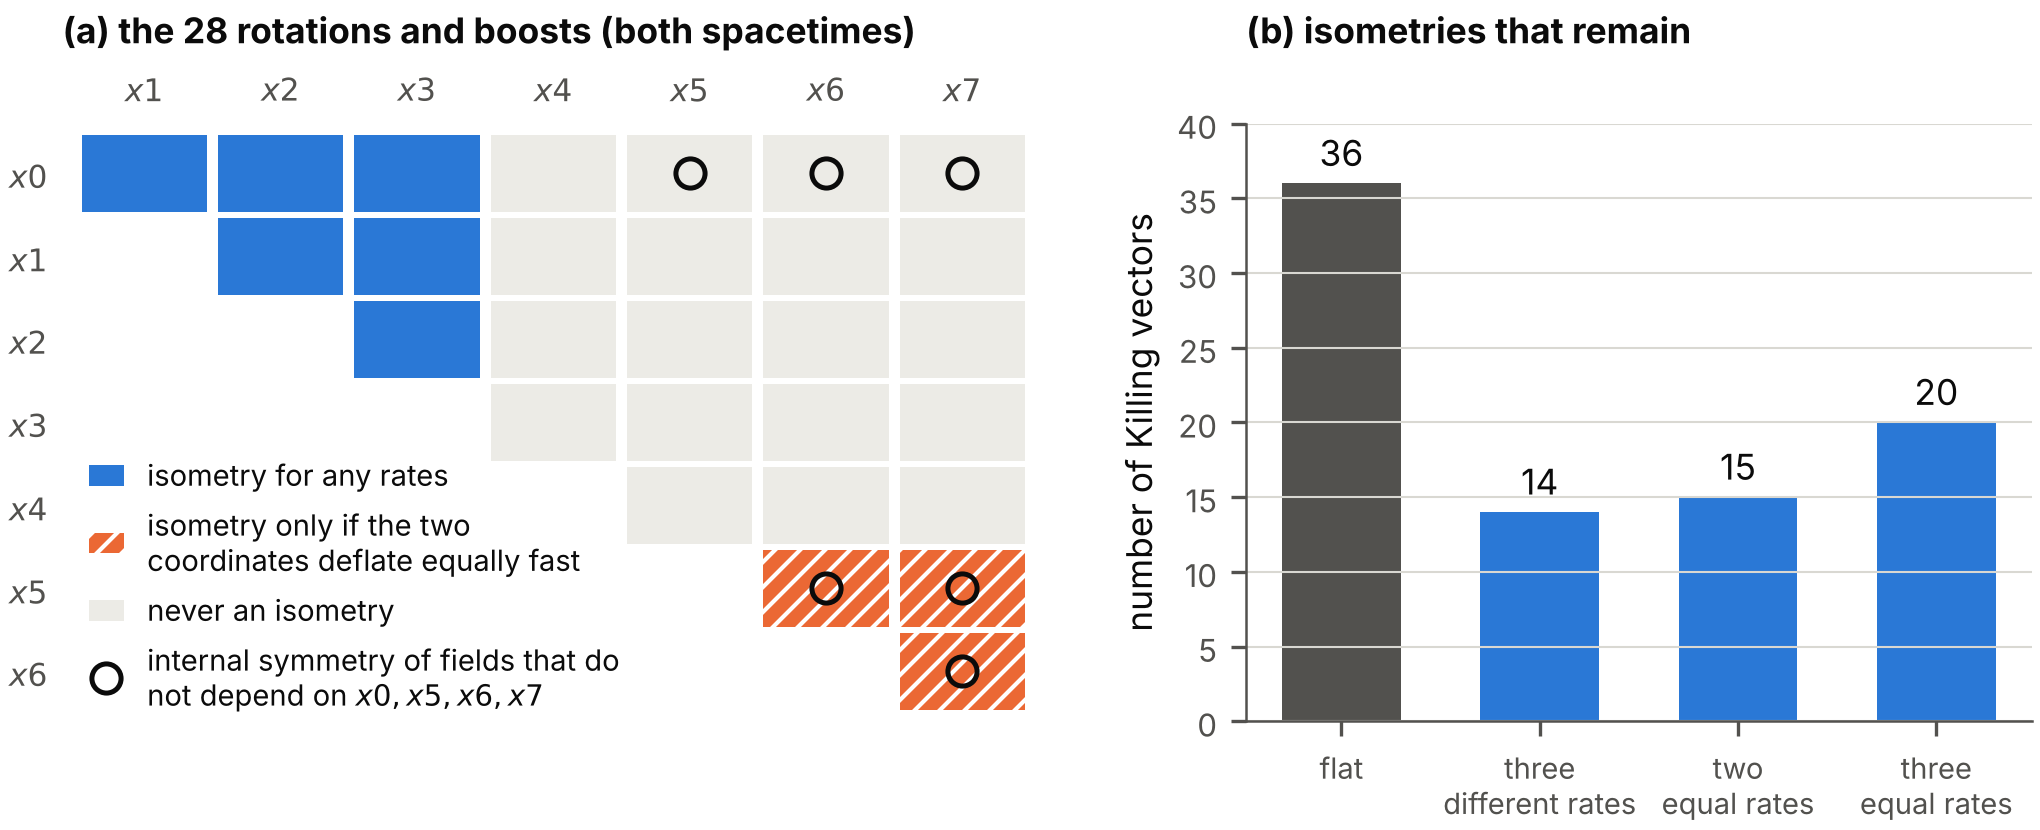
\includegraphics[width=1\textwidth,height=\textheight]{../figures/fig_isometries.png}
\caption{The 28 rotations and boosts on the deflating spacetimes, and
the number of Killing vectors (the figure of DMD, Sec. 1.5). The circles
mark the six internal generators: for three different rates none of them
is a symmetry of the spacetime. Data: \texttt{data/isometries.csv};
program: \texttt{deflation\ symmetry}.}
\end{figure}

\begin{center}\rule{0.5\linewidth}{0.5pt}\end{center}

\hypertarget{condition-c2-a-condensate-in-empty-space}{%
\section{4. Condition C2: a condensate in empty
space}\label{condition-c2-a-condensate-in-empty-space}}

S2 leaves C2 open: by the ladder equation of the supplement S4 a pair
condensate forms in the vacuum only if \(\alpha_{VS}\) exceeds a
critical value \(\alpha_c\) of about 2 or more, depending on the cutoff.
On a deflating spacetime \(\alpha_{VS}\) grows as \(e^{\tau_d}\) and
reaches any such value at a definite time. The supplement RS4, Sec. 5,
shows what else has happened by then: for \(\alpha_{VS}\) of order one
the one-boson exchange is no longer a controlled approximation, and the
field at which the one-loop potential of the Vorton-Scalar falls below
its vacuum value has moved to within a factor of two of the vacuum
value. \textbf{C2 can be reached by waiting, but not within the range of
validity of the model.} The status of C2 remains ``open''.

\begin{center}\rule{0.5\linewidth}{0.5pt}\end{center}

\hypertarget{a-new-condition-the-electroweak-scale-must-not-drift}{%
\section{5. A new condition: the electroweak scale must not
drift}\label{a-new-condition-the-electroweak-scale-must-not-drift}}

\hypertarget{the-argument}{%
\subsection{5.1 The argument}\label{the-argument}}

Suppose H2 holds. The electroweak scale \(v_{\rm EW}\) is then the scale
of the pair condensate in the vacuum. That scale is determined by the
parameters of the model: the masses \(m\) and \(m_s\), the cutoff, and
the coupling \(\alpha_{VS}\). On the deflating spacetime the masses are
constant and \(\alpha_{VS}\propto e^{\tau_d}\) (RS1, Sec. 1.3).
Therefore
\[v_{\rm EW}\ \propto\ e^{\,n_{\rm EW}\,\tau_d},\qquad n_{\rm EW}=\frac{d\ln v_{\rm EW}}{d\ln\alpha_{VS}} .\tag{5.1}\]
The exponent cannot vanish: below the critical coupling there is no
condensate, so the scale depends on the coupling, and most strongly just
above the critical coupling.

\emph{What follows for ordinary matter.} Under H2 the masses of the
electron and of the quarks are proportional to \(v_{\rm EW}\) and change
at the rate \(n_{\rm EW}\,\mathrm{gsum}\). The mass of the proton is due
mostly to the strong interaction and does not follow. The ratio
\(m_p/m_e\) of the two masses therefore changes at the rate
\(n_{\rm EW}\,\mathrm{gsum}\). Comparisons of atomic clocks find this
ratio constant to \(8.0\times10^{-17}\) per year at two sigma (Ref.
{[}1{]}). Hence
\[\boxed{\;\mathrm{gsum}<\frac{8.0\times10^{-17}\ \text{per year}}{n_{\rm EW}}=\frac{1.16\times10^{-6}\,H_0}{n_{\rm EW}}\;}\tag{5.2}\]
(check \texttt{def-C6}). The bound needs no assumption about gravity.
For \(n_{\rm EW}=1\) it is 2787 times stronger than the bound that lunar
laser ranging gives if gravity is eight-dimensional (RS3, Sec. 3).

\hypertarget{the-size-of-the-exponent}{%
\subsection{5.2 The size of the
exponent}\label{the-size-of-the-exponent}}

For the model itself --- massive fermions and a massive radial mode ---
the scale of the vacuum condensate has not been computed as a function
of the coupling. It is known in closed form for the case on which S4
tests its ladder equation: massless fermions and massless bosons between
an infrared scale and a cutoff. There the scale of the condensate obeys
\[\varrho_c\,\ln\frac{\text{cutoff}}{\text{scale}}=\arctan\frac{1}{2\varrho_c},\qquad
\varrho_c^2=\frac14\Big(\frac{\alpha_{VS}}{\alpha_c}-1\Big),\] (the
relation of S4, Sec. 7.2, written with the ratio of the coupling to its
critical value; \(\varrho_c\) is only an abbreviation for the square
root on the right), from which
\[n_{\rm EW}=\frac{(1+4\varrho_c^2)\,\arctan(1/2\varrho_c)}{8\,\varrho_c^3}+\frac{1}{4\varrho_c^2} .\tag{5.3}\]
The program verifies Eq. (5.3) against the numerical derivative to
\(3\times10^{-8}\) and tabulates it, together with the bound (5.2):

\begin{longtable}[]{@{}
  >{\raggedleft\arraybackslash}p{(\columnwidth - 8\tabcolsep) * \real{0.2000}}
  >{\raggedleft\arraybackslash}p{(\columnwidth - 8\tabcolsep) * \real{0.2000}}
  >{\raggedleft\arraybackslash}p{(\columnwidth - 8\tabcolsep) * \real{0.2000}}
  >{\raggedleft\arraybackslash}p{(\columnwidth - 8\tabcolsep) * \real{0.2000}}
  >{\raggedleft\arraybackslash}p{(\columnwidth - 8\tabcolsep) * \real{0.2000}}@{}}
\toprule\noalign{}
\begin{minipage}[b]{\linewidth}\raggedleft
\(\alpha_{VS}/\alpha_c\)
\end{minipage} & \begin{minipage}[b]{\linewidth}\raggedleft
\(\ln\)(cutoff/scale)
\end{minipage} & \begin{minipage}[b]{\linewidth}\raggedleft
\(n_{\rm EW}\)
\end{minipage} & \begin{minipage}[b]{\linewidth}\raggedleft
bound on gsum (per year)
\end{minipage} & \begin{minipage}[b]{\linewidth}\raggedleft
bound in units of \(H_0\)
\end{minipage} \\
\midrule\noalign{}
\endhead
\bottomrule\noalign{}
\endlastfoot
1.05 & 12.082 & 147 & \(5.4\times10^{-19}\) & \(7.9\times10^{-9}\) \\
1.10 & 7.998 & 54.0 & \(1.5\times10^{-18}\) & \(2.2\times10^{-8}\) \\
1.25 & 4.429 & 15.1 & \(5.3\times10^{-18}\) & \(7.7\times10^{-8}\) \\
1.50 & 2.702 & 6.05 & \(1.3\times10^{-17}\) & \(1.9\times10^{-7}\) \\
2.00 & 1.571 & 2.57 & \(3.1\times10^{-17}\) & \(4.5\times10^{-7}\) \\
3.00 & 0.870 & 1.15 & \(6.9\times10^{-17}\) & \(1.0\times10^{-6}\) \\
5.00 & 0.464 & 0.540 & \(1.5\times10^{-16}\) & \(2.2\times10^{-6}\) \\
10.0 & 0.215 & 0.230 & \(3.5\times10^{-16}\) & \(5.0\times10^{-6}\) \\
\end{longtable}

The exponent diverges at the critical coupling, equals \(1+\pi/2=2.57\)
at twice the critical coupling, and exceeds 1 for
\(\alpha_{VS}<3.27\,\alpha_c\). It falls below 1 only where the scale of
the condensate approaches the cutoff, that is, where the
four-dimensional description ends. \emph{Within the range in which a
condensate of the kind that H2 needs can be described at all,
\(n_{\rm EW}\) is of order one or larger.}

\hypertarget{the-conclusion}{%
\subsection{5.3 The conclusion}\label{the-conclusion}}

By Eq. (5.2), under H2 the deflation clock can have advanced by at most
\(\mathrm{gsum}\,t_0<1.1\times10^{-6}/n_{\rm EW}\) during the age
\(t_0\) of the universe at a constant rate. Every effect of the
deflation described in the supplements RS1, RS3 and RS4 is then
unobservably small. Conversely, a deflation at any rate that those
supplements find interesting excludes H2.

This conclusion does not depend on the unresolved conditions C2 and C5
to C7. It depends on two properties only: that the electroweak scale is
set by the dynamics of the model, and that the coupling of the model
follows the volume of the deflating coordinates. The first is the
content of H2; the second is exact (RS1, Sec. 1).

\begin{figure}
\centering
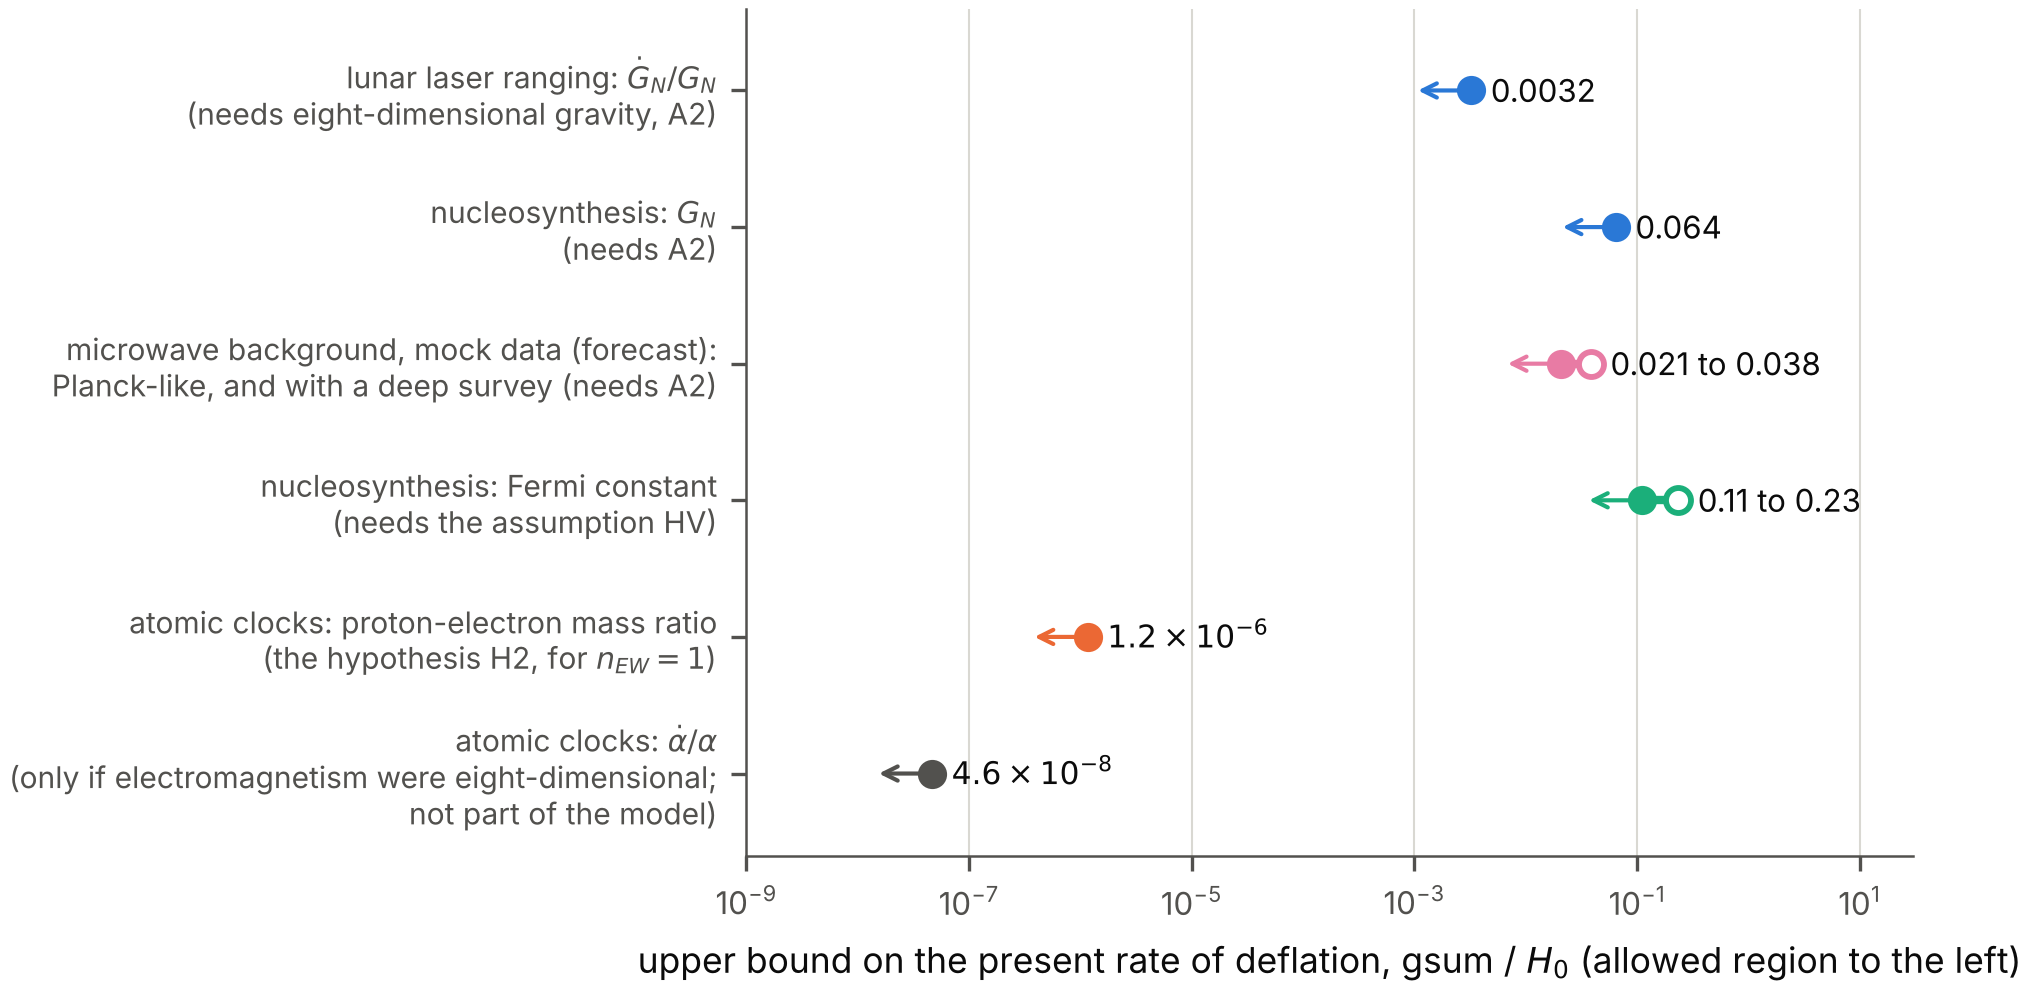
\includegraphics[width=1\textwidth,height=\textheight]{../figures/fig_bounds.png}
\caption{Upper bounds on the present rate of deflation (the figure of
RS3, Sec. 3). The bound that follows from the hypothesis H2 and the
atomic clocks, Eq. (5.2) with \(n_{\rm EW}=1\), is the fourth from the
top. Data: \texttt{data/deflation\_bounds.csv}; program:
\texttt{deflation\ cosmology}.}
\end{figure}

\begin{center}\rule{0.5\linewidth}{0.5pt}\end{center}

\hypertarget{verdict}{%
\section{6. Verdict}\label{verdict}}

\begin{longtable}[]{@{}
  >{\raggedright\arraybackslash}p{(\columnwidth - 6\tabcolsep) * \real{0.2500}}
  >{\raggedright\arraybackslash}p{(\columnwidth - 6\tabcolsep) * \real{0.2609}}
  >{\raggedright\arraybackslash}p{(\columnwidth - 6\tabcolsep) * \real{0.2609}}
  >{\raggedright\arraybackslash}p{(\columnwidth - 6\tabcolsep) * \real{0.2283}}@{}}
\toprule\noalign{}
\begin{minipage}[b]{\linewidth}\raggedright
Condition
\end{minipage} & \begin{minipage}[b]{\linewidth}\raggedright
deflating 7+1
\end{minipage} & \begin{minipage}[b]{\linewidth}\raggedright
deflating 4+4
\end{minipage} & \begin{minipage}[b]{\linewidth}\raggedright
Basis
\end{minipage} \\
\midrule\noalign{}
\endhead
\bottomrule\noalign{}
\endlastfoot
C1 scalar in ordinary spacetime & met in the sector & met in the sector
& Sec. 2; check \texttt{def-S3} \\
C2 condensate in the vacuum & open; reached in time only outside the
range of validity & the same & Sec. 4; RS4, Sec. 5 \\
C3 doublet with a neutral component & only under a hidden symmetry
(three different rates), or with \(SO(3)\) alone as a symmetry of the
spacetime (equal rates) & only under a hidden symmetry; singlet under
\(SO(3)_T\) & Sec. 3; checks \texttt{71d-S2}, \texttt{44d-S2} \\
C4 breaking \(SO(4)\to SO(3)\) & met in the sector; the spacetime itself
has at most the \(SO(3)\) & met in the sector only & Secs. 2, 3 \\
C5 scale and scalar mass & unfavourable (estimate of S2, unchanged) &
--- & S2, Sec. 5 \\
C6 masses of ordinary fermions & not addressed & --- & S2, Sec. 5 \\
C7 no unobserved particles & additional particles predicted & --- & S2,
Sec. 5 \\
\textbf{new:} the electroweak scale does not drift & requires
\(\mathrm{gsum}<1.16\times10^{-6}H_0/n_{\rm EW}\) & the same & Sec. 5;
check \texttt{def-C6} \\
\end{longtable}

\textbf{What has been established.}

\begin{enumerate}
\def\labelenumi{\arabic{enumi}.}
\tightlist
\item
  The internal symmetry of the sector of fields that do not depend on
  the extra coordinates, the representation of the pair operators and
  the breaking pattern are unchanged by the deflation (Sec. 2).
\item
  Of the six generators of that symmetry, the deflating spacetime keeps
  none, one or three as symmetries of the spacetime; the three that mix
  the hidden axis with a deflating coordinate are never symmetries (Sec.
  3). On the deflating 7+1 spacetime the structural point that S2
  counted in favour of the hypothesis survives only for a hidden
  symmetry.
\item
  Under H2 the electroweak scale follows the coupling with the exponent
  \(n_{\rm EW}\), and atomic clocks bound the rate of deflation by Eq.
  (5.2). \(n_{\rm EW}\) is given in closed form for the scale-invariant
  ladder equation (Sec. 5).
\end{enumerate}

\textbf{What has not been established.}

\begin{enumerate}
\def\labelenumi{\arabic{enumi}.}
\tightlist
\item
  Everything that S2 lists as not established: that a vacuum condensate
  forms, that rotations of extra dimensions are the electroweak gauge
  group, the scale and the mass of the scalar, the masses of ordinary
  fermions.
\item
  The exponent \(n_{\rm EW}\) for the model itself. Eq. (5.3) holds for
  massless fermions and bosons; the statement that \(n_{\rm EW}\) is of
  order one or larger rests on that case and on the general fact that
  the scale vanishes at the critical coupling.
\item
  Whether a mechanism exists that would make the electroweak scale
  insensitive to the coupling of the pair. None is known in the model.
\end{enumerate}

The hypothesis ``the singlet superfluid is the Higgs field'' is
therefore, on the deflating spacetimes, \textbf{unproven, with less in
its favour than on the flat 7+1 spacetime, and incompatible with any
deflation that is fast enough to matter today.}

\begin{center}\rule{0.5\linewidth}{0.5pt}\end{center}

\hypertarget{appendix-a.-output-of-the-programs}{%
\section{Appendix A. Output of the
programs}\label{appendix-a.-output-of-the-programs}}

\hypertarget{a.1-deflation-symmetry}{%
\subsection{\texorpdfstring{A.1
\texttt{deflation\ symmetry}}{A.1 deflation symmetry}}\label{a.1-deflation-symmetry}}

\begin{Shaded}
\begin{Highlighting}[]
\NormalTok{PROJECT spacetimes, Revision\_Deflation: checks of the symmetries on the deflating spacetimes (isometries, internal symmetry of the fields that do not depend on the extra coordinates, zero modes on a vortex line, reduction of the couplings)}
\NormalTok{generated by: deflation (Rust crate spacetimes{-}deflation, version 0.1.0; PROJECT spacetimes, Revision\_Deflation); command: deflation symmetry}
\NormalTok{18 of 18 checks passed}

\NormalTok{[PASS] 44d{-}S1  (exact) of the 28 rotations and boosts of the flat 4+4 spacetime (one for each pair of coordinates) exactly 6 remain isometries of the deflating spacetime for three different rates (the rotations of x0, x1, x2, x3), 7 if two rates are equal (in addition the rotation of the two coordinates that deflate at the same rate) and 9 if the three rates are equal (in addition the three rotations of x5, x6, x7); no transformation that involves x4 survives, and none that mixes x0 with a deflating coordinate. Together with the 7 translations, the scaling and, for equal rates, the three special vectors of metric.rs this gives 14, 15 and 20 Killing vectors (Lie derivative of the metric zero at two points, exact arithmetic)}
\NormalTok{[PASS] 44d{-}S2  (exact) the products gamma\^{}A gamma\^{}B that commute with the five matrices alpha\^{}1, alpha\^{}2, alpha\^{}3, beta, i beta chi (and so act as internal symmetries on fields that do not depend on the extra coordinates) are exactly those of the six pairs taken from x0, x5, x6, x7. Of these six, the deflating spacetime keeps as isometries 0 (three different rates), 1 (two equal rates) and 3 (three equal rates): the remaining 6, 5 and 3 are symmetries of the sector of such fields that have no counterpart among the isometries of the spacetime (hidden symmetries)}
\NormalTok{[PASS] 71d{-}S1  (exact) of the 28 rotations and boosts of the flat 7+1 spacetime (one for each pair of coordinates) exactly 6 remain isometries of the deflating spacetime for three different rates (the rotations of x0, x1, x2, x3), 7 if two rates are equal (in addition the rotation of the two coordinates that deflate at the same rate) and 9 if the three rates are equal (in addition the three rotations of x5, x6, x7); no transformation that involves x4 survives, and none that mixes x0 with a deflating coordinate. Together with the 7 translations, the scaling and, for equal rates, the three special vectors of metric.rs this gives 14, 15 and 20 Killing vectors (Lie derivative of the metric zero at two points, exact arithmetic)}
\NormalTok{[PASS] 71d{-}S2  (exact) the products gamma\^{}A gamma\^{}B that commute with the five matrices alpha\^{}1, alpha\^{}2, alpha\^{}3, beta, i beta chi (and so act as internal symmetries on fields that do not depend on the extra coordinates) are exactly those of the six pairs taken from x0, x5, x6, x7. Of these six, the deflating spacetime keeps as isometries 0 (three different rates), 1 (two equal rates) and 3 (three equal rates): the remaining 6, 5 and 3 are symmetries of the sector of such fields that have no counterpart among the isometries of the spacetime (hidden symmetries)}
\NormalTok{[PASS] def{-}S3  (numerical) the internal symmetry of the fields that do not depend on the extra coordinates, computed again for both spacetimes (24 items of data/reduced\_symmetry.csv, all as expected): the commutant of the five matrices has dimension 8 and is u(2) + u(2) = su(2)\_A + su(2)\_B + u(1)\_F + u(1)\_E; the eight one{-}particle states are (2,1) + (1,2); the four vector pair operators are the (2,2) with fermion number 2, and their invariant quadratic form is the frame metric of the axes x0, x5, x6, x7. The deflation does not change this symmetry, because the weighted field of this sector obeys the flat equations (checks 44d{-}D.., 71d{-}D.. of the command matrices)}
\NormalTok{[PASS] 44d{-}V1  (exact) alpha\^{}1, alpha\^{}2, alpha\^{}3, beta and i beta chi are Hermitian, have square one and anticommute with one another}
\NormalTok{[PASS] 44d{-}V2  (exact) i beta alpha\^{}1 and alpha\^{}2 beta chi are commuting Hermitian matrices with square one}
\NormalTok{[PASS] 44d{-}V3  (exact) each of the four joint eigenspaces of the two matrices has dimension 4: a vortex line of unit winding carries four zero modes of the sixteen{-}component field}
\NormalTok{[PASS] 44d{-}V4  (exact) Pc = i alpha\^{}1 alpha\^{}2 alpha\^{}3 chi equals the product of the five matrices, commutes with each of them, is Hermitian and traceless and has square one: it is, up to sign, the generator P of U(1)\_E}
\NormalTok{[PASS] 44d{-}V5  (exact) winding +1: every w\_z with (i beta alpha\^{}1) w\_z = {-}w\_z, (alpha\^{}2 beta chi) w\_z = {-}w\_z solves the zero{-}energy equations (i alpha\^{}1 + beta) w\_z = 0, (i alpha\^{}2 + i beta chi) w\_z = 0; on these four spinors alpha\^{}3 = Pc, and its trace vanishes: two zero modes have alpha\^{}3 = +1 (energy +k\_3) and two alpha\^{}3 = {-}1 (energy {-}k\_3)}
\NormalTok{[PASS] 44d{-}V6  (exact) winding {-}1: the spinors w\_z with (i beta alpha\^{}1) w\_z = {-}w\_z, (alpha\^{}2 beta chi) w\_z = +w\_z solve (i alpha\^{}1 + beta) w\_z = 0, (i alpha\^{}2 {-} i beta chi) w\_z = 0, and on them alpha\^{}3 = {-}Pc: the directions of motion are exchanged}
\NormalTok{[PASS] 71d{-}V1  (exact) alpha\^{}1, alpha\^{}2, alpha\^{}3, beta and i beta chi are Hermitian, have square one and anticommute with one another}
\NormalTok{[PASS] 71d{-}V2  (exact) i beta alpha\^{}1 and alpha\^{}2 beta chi are commuting Hermitian matrices with square one}
\NormalTok{[PASS] 71d{-}V3  (exact) each of the four joint eigenspaces of the two matrices has dimension 4: a vortex line of unit winding carries four zero modes of the sixteen{-}component field}
\NormalTok{[PASS] 71d{-}V4  (exact) Pc = i alpha\^{}1 alpha\^{}2 alpha\^{}3 chi equals the product of the five matrices, commutes with each of them, is Hermitian and traceless and has square one: it is, up to sign, the generator P of U(1)\_E}
\NormalTok{[PASS] 71d{-}V5  (exact) winding +1: every w\_z with (i beta alpha\^{}1) w\_z = {-}w\_z, (alpha\^{}2 beta chi) w\_z = {-}w\_z solves the zero{-}energy equations (i alpha\^{}1 + beta) w\_z = 0, (i alpha\^{}2 + i beta chi) w\_z = 0; on these four spinors alpha\^{}3 = Pc, and its trace vanishes: two zero modes have alpha\^{}3 = +1 (energy +k\_3) and two alpha\^{}3 = {-}1 (energy {-}k\_3)}
\NormalTok{[PASS] 71d{-}V6  (exact) winding {-}1: the spinors w\_z with (i beta alpha\^{}1) w\_z = {-}w\_z, (alpha\^{}2 beta chi) w\_z = +w\_z solve (i alpha\^{}1 + beta) w\_z = 0, (i alpha\^{}2 {-} i beta chi) w\_z = 0, and on them alpha\^{}3 = {-}Pc: the directions of motion are exchanged}
\NormalTok{[PASS] def{-}S4  (exact) reduction to fields that do not depend on x5, x6, x7: sqrt|g| times the Yukawa term and the potential of the Vorton{-}Scalar, written with the weighted fields psihat = sqrt(Vd) psi and Phihat = sqrt(Vd) Phi\_VS, are the same expressions with the couplings y\_VS/sqrt(Vd), lambda\_VS/Vd and the vacuum value v\_VS sqrt(Vd); the products y\_VS v\_VS and lambda\_VS v\_VS\^{}2, hence the fermion mass and the mass of the radial mode, do not change (rational sample values, exact). The exponents of data/coupling\_exponents.csv follow, with Vd proportional to exp({-}gsum x4)}
\NormalTok{[PASS] ALL  (exact) every check above passed}
\end{Highlighting}
\end{Shaded}

\hypertarget{a.2-deflation-cosmology}{%
\subsection{\texorpdfstring{A.2
\texttt{deflation\ cosmology}}{A.2 deflation cosmology}}\label{a.2-deflation-cosmology}}

\begin{Shaded}
\begin{Highlighting}[]
\NormalTok{PROJECT spacetimes, Revision\_Deflation: checks of the cosmological calculations on the deflating spacetime}
\NormalTok{generated by: deflation (Rust crate spacetimes{-}deflation, version 0.1.0; PROJECT spacetimes, Revision\_Deflation); command: deflation cosmology}
\NormalTok{6 of 6 checks passed}

\NormalTok{[PASS] def{-}C1  (numerical) without deflation the background integrals of this module agree with the main project (its recombination calculation gives z\_* = 1089.92): 100 theta\_* = 1.03965 here against 1.03965, sound horizon 144.449 Mpc against 144.449 Mpc; age 13.814 Gyr}
\NormalTok{[PASS] def{-}C2  (numerical) with deflation at a constant rate, gravity was weaker in the past, the early universe expanded more slowly at a given density, and the sound horizon is larger; holding 100 theta\_*, omega\_b and omega\_c fixed, the inferred Hubble constant FALLS monotonically with the rate: d ln H\_0/d(gsum/H\_0) = {-}0.969 at small rates; H\_0 = 66.70, 65.36, 60.37 km/s/Mpc for gsum = 0.01, 0.03, 0.1 H\_0 (67.36 without deflation). Deflation moves the Hubble constant away from the locally measured value. These numbers come from the full calculation of recombination on the deflating background (last scattering moves from z\_* = 1089.92 to 1088.04 at gsum = 0.1 H\_0, and the helium fraction falls). If z\_* and the helium fraction are held at their values without deflation, the slope is {-}0.911 and the values are 66.74, 65.48, 60.77 km/s/Mpc: that approximation underestimates the fall by 5.8 to 6.0 per cent}
\NormalTok{[PASS] def{-}C3  (numerical) bounds on the present rate of deflation if gravity is eight{-}dimensional (G\_N grows at the rate gsum): lunar laser ranging, (dG\_N/dt)/G\_N = (7.1 +{-} 7.6) 10\^{}{-}14 per year, gives gsum \textless{} 2.23e{-}13 per year = 3.24e{-}3 H\_0 at two sigma; nucleosynthesis, G\_N(nucleosynthesis)/G\_N(today) \textgreater{} 0.94 at two sigma, gives gsum \textless{} 4.43e{-}12 per year = 0.064 H\_0 for a rate that was constant since then. At these rates the inferred Hubble constant changes by {-}0.211 and {-}4.38 km/s/Mpc, in the direction away from the local measurement, 73.50 +{-} 0.81 km/s/Mpc. Over the age t\_0 of the model without deflation (H\_0 t\_0 = 0.9516) the deflation clock has advanced by gsum t\_0 = 3.1e{-}3 at the first of these rates}
\NormalTok{[PASS] def{-}C5  (numerical) bounds that do not rest on gravity: (i) under the assumption HV (the vacuum value of the Vorton{-}Scalar sets the electroweak scale) the Fermi constant grows at the rate gsum while every mass stays constant; nucleosynthesis with fixed masses allows G\_Fermi at t = 1 s to differ by 10 to 20 per cent from today\textquotesingle{}s value (Scherrer and Spergel 1993), which gives gsum \textless{} 0.111 to 0.234 H\_0, weaker than the bound from Newton\textquotesingle{}s constant; (ii) in the model as it stands (without H2 and without HV) no mass of ordinary matter depends on the deflation, and the measured constancy of the ratio of the proton mass to the electron mass does not bound the rate; (iii) the fine{-}structure constant would bound it, gsum \textless{} 3.2e{-}18 per year = 4.6e{-}8 H\_0, only if the electromagnetic field propagated along the deflating coordinates, which is not part of the model}
\NormalTok{[PASS] def{-}C6  (numerical) the author\textquotesingle{}s hypothesis H2 (the superfluid state is the Higgs field) on a deflating spacetime: the electroweak scale is then the scale of the pair condensate, which depends on alpha\_VS, and alpha\_VS grows as exp(gsum x4). With n\_EW = d ln v\_EW/d ln alpha\_VS the electron mass changes at the rate n\_EW gsum and the proton mass does not; atomic clocks (ratio of the two masses constant to 8.0e{-}17 per year at two sigma) then give gsum \textless{} 8.0e{-}17 per year / n\_EW = 1.16e{-}6 H\_0 / n\_EW, a bound 2787 times stronger than that of lunar laser ranging for n\_EW = 1, and one that needs no assumption about gravity; over the age of the universe the deflation clock can then have advanced by at most 1.1e{-}6/n\_EW. In the scale{-}invariant ladder equation of the main project n\_EW = (1 + 4 rho\_c\^{}2) atan(1/(2 rho\_c))/(8 rho\_c\^{}3) + 1/(4 rho\_c\^{}2) with rho\_c\^{}2 = (alpha\_VS/alpha\_c {-} 1)/4 (agreement with the numerical derivative: 2.8e{-}8): n\_EW = 15.1, 2.57, 1.15, 0.54 for alpha\_VS/alpha\_c = 1.25, 2, 3, 5; it diverges at the critical coupling and exceeds 1 for alpha\_VS \textless{} 3.27 alpha\_c. For the model itself (massive fermions, massive radial mode) n\_EW has not been computed}
\NormalTok{[PASS] def{-}C4  (numerical) dark matter of bound pairs loses rest mass while the coupling grows, because the binding energy increases (four examples with alpha\_VS = 0.4 to 1 today; binding energy at most 8.2 per cent of the rest mass). If gravity feels the deflation, the inferred Hubble constant changes by between {-}4.11 and {-}0.19 km/s/Mpc at the rates that lunar laser ranging and nucleosynthesis allow: it falls, the weaker gravity of the past outweighing the loss of mass. (The runs with a varying rest mass hold the redshift of last scattering and the helium fraction at their values without deflation, which by def{-}C2 underestimates a fall by about six per cent of itself.) If Newton\textquotesingle{}s constant is held fixed and the deflation acts on the dark sector alone, rates between 0.03 and 1 H\_0 change the inferred Hubble constant by at most +0.48 km/s/Mpc, for a loss of up to 7.7 per cent of the rest mass (data/hubble\_mass\_loss.csv). The loss of rest mass is the only effect of the deflation that raises the inferred Hubble constant; in these examples it supplies less than a tenth of the 6.1 km/s/Mpc that separate 67.36 from the local value 73.50}
\NormalTok{[PASS] ALL  (numerical) every check above passed}
\end{Highlighting}
\end{Shaded}

\hypertarget{appendix-b.-the-internal-symmetry-of-the-sector-item-by-item}{%
\section{Appendix B. The internal symmetry of the sector, item by
item}\label{appendix-b.-the-internal-symmetry-of-the-sector-item-by-item}}

The 24 items of \texttt{data/reduced\_symmetry.csv}, as the program
writes them (check \texttt{def-S3}). The symbols in this table are those
of the main registry: \(P\) is the generator of \(U(1)_E\), \(T_i\) are
the generators of the two ideals \(su(2)_A\) and \(su(2)_B\), and
\(C^-\gamma^a\) are the matrices of the four vector pair operators.

\begin{longtable}[]{@{}
  >{\raggedright\arraybackslash}p{(\columnwidth - 6\tabcolsep) * \real{0.4783}}
  >{\raggedleft\arraybackslash}p{(\columnwidth - 6\tabcolsep) * \real{0.1739}}
  >{\raggedleft\arraybackslash}p{(\columnwidth - 6\tabcolsep) * \real{0.1739}}
  >{\raggedleft\arraybackslash}p{(\columnwidth - 6\tabcolsep) * \real{0.1739}}@{}}
\toprule\noalign{}
\begin{minipage}[b]{\linewidth}\raggedright
item
\end{minipage} & \begin{minipage}[b]{\linewidth}\raggedleft
7+1
\end{minipage} & \begin{minipage}[b]{\linewidth}\raggedleft
4+4
\end{minipage} & \begin{minipage}[b]{\linewidth}\raggedleft
expected
\end{minipage} \\
\midrule\noalign{}
\endhead
\bottomrule\noalign{}
\endlastfoot
dimension of the commutant, momenta along x1 x2 x3 & 8 & 8 & 8 \\
dimension of the commutant, momenta along x0 x1 x2 x3 & 4 & 4 & 4 \\
dimension of the commutant, momenta along every space coordinate of the
model & 1 & 4 & 1 (7+1); 4 (4+4) \\
dimension of the centre of the commutant & 2 & 2 & 2 \\
\textbar P\^{}2 - 1\textbar{} for the traceless central generator P &
0.00e0 & 0.00e0 & 0 \\
dimensions of the two ideals & {[}3, 3{]} & {[}3, 3{]} & {[}3, 3{]} \\
structure constants \textbar f\_123\textbar{} of the ideals (generators
with Tr T\_i T\_j = 2 delta\_ij) & 1.000000000000 1.000000000000 &
1.000000000000 1.000000000000 & 1 1 (su(2)) \\
\textbar sum\_i T\_i\^{}2 - (3/4) projector\textbar{} of the ideals &
0.00e0 0.00e0 & 2.22e-16 2.22e-16 & 0 0 (doublets) \\
positive-energy states with P = +1 and P = -1 at a test momentum &
4.000000 4.000000 & 4.000000 4.000000 & 4 4: (2,1) + (1,2) \\
closure of the four vector pair operators C\^{}- gamma\^{}a, a in
\{0,5,6,7\} & 0.00e0 & 3.14e-16 & 0 \\
\textbar Casimir - 3/4\textbar{} of the two ideals on the four pair
operators & 0.00e0 0.00e0 & 5.55e-17 5.55e-17 & 0 0: the (2,2) \\
fermion number of the pair operators & 2.000000 & 2.000000 & 2 \\
charge of the pair operators under the central generator P & 0.00e0 &
0.00e0 & 0 \\
number of invariant quadratic forms on the four pair operators & 1 & 1 &
1 \\
the invariant form (diagonal; frame axes 0 5 6 7; first entry 1) &
+1.000000 +1.000000 +1.000000 +1.000000 & +1.000000 -1.000000 -1.000000
-1.000000 & +1 +1 +1 +1 (7+1); +1 -1 -1 -1 (4+4): the frame metric of
the extra axes up to sign \\
largest off-diagonal entry of the invariant form & 0.00e0 & 2.22e-16 &
0 \\
complex dimension of the particle-antiparticle mixing generators, no
chemical potential & 2 & 2 & 2 (symmetry O(4) x O(4), dimension 12) \\
the same with a chemical potential & 0 & 0 & 0 (symmetry U(2) x U(2),
dimension 8) \\
gamma\^{}0 gamma\^{}5 & antihermitian;
\textbar{[}.,dynamics{]}\textbar{} = 0.00e0 & Hermitian;
\textbar{[}.,dynamics{]}\textbar{} = 0.00e0 & antihermitian (7+1:
rotation); Hermitian (4+4: not a boost); commutes \\
gamma\^{}0 gamma\^{}6 & antihermitian;
\textbar{[}.,dynamics{]}\textbar{} = 0.00e0 & Hermitian;
\textbar{[}.,dynamics{]}\textbar{} = 0.00e0 & antihermitian (7+1:
rotation); Hermitian (4+4: not a boost); commutes \\
gamma\^{}0 gamma\^{}7 & antihermitian;
\textbar{[}.,dynamics{]}\textbar{} = 0.00e0 & Hermitian;
\textbar{[}.,dynamics{]}\textbar{} = 0.00e0 & antihermitian (7+1:
rotation); Hermitian (4+4: not a boost); commutes \\
gamma\^{}5 gamma\^{}6 & antihermitian;
\textbar{[}.,dynamics{]}\textbar{} = 0.00e0 & antihermitian;
\textbar{[}.,dynamics{]}\textbar{} = 0.00e0 & antihermitian (rotation)
in both; commutes \\
gamma\^{}5 gamma\^{}7 & antihermitian;
\textbar{[}.,dynamics{]}\textbar{} = 0.00e0 & antihermitian;
\textbar{[}.,dynamics{]}\textbar{} = 0.00e0 & antihermitian (rotation)
in both; commutes \\
gamma\^{}6 gamma\^{}7 & antihermitian;
\textbar{[}.,dynamics{]}\textbar{} = 0.00e0 & antihermitian;
\textbar{[}.,dynamics{]}\textbar{} = 0.00e0 & antihermitian (rotation)
in both; commutes \\
\end{longtable}

\hypertarget{appendix-c.-files}{%
\section{Appendix C. Files}\label{appendix-c.-files}}

\begin{longtable}[]{@{}
  >{\raggedright\arraybackslash}p{(\columnwidth - 4\tabcolsep) * \real{0.1905}}
  >{\raggedright\arraybackslash}p{(\columnwidth - 4\tabcolsep) * \real{0.6190}}
  >{\raggedright\arraybackslash}p{(\columnwidth - 4\tabcolsep) * \real{0.1905}}@{}}
\toprule\noalign{}
\begin{minipage}[b]{\linewidth}\raggedright
file
\end{minipage} & \begin{minipage}[b]{\linewidth}\raggedright
content
\end{minipage} & \begin{minipage}[b]{\linewidth}\raggedright
written by
\end{minipage} \\
\midrule\noalign{}
\endhead
\bottomrule\noalign{}
\endlastfoot
\texttt{code/deflation-rs/src/symmetry\_defl.rs},
\texttt{cmd\_symmetry.rs} & test of the 28 rotations and boosts;
internal symmetry of the sector & --- \\
\texttt{data/isometries.csv} & Sec. 3 & \texttt{deflation\ symmetry} \\
\texttt{data/reduced\_symmetry.csv} & Sec. 2 and Appendix B &
\texttt{deflation\ symmetry} \\
\texttt{data/higgs\_scale\_exponent.csv},
\texttt{data/deflation\_bounds.csv} & Sec. 5 &
\texttt{deflation\ cosmology} \\
\texttt{data/symmetry\_checks.txt}, \texttt{data/cosmology\_checks.txt}
(and \texttt{.csv}) & Appendix A & the two commands \\
\texttt{figures/fig\_isometries}, \texttt{figures/fig\_bounds}
(\texttt{.pdf}, \texttt{.png}) & the two figures &
\texttt{make\_figures.py} \\
\end{longtable}

\hypertarget{references}{%
\section{References}\label{references}}

\begin{enumerate}
\def\labelenumi{\arabic{enumi}.}
\tightlist
\item
  R. Lange, N. Huntemann, J. M. Rahm, C. Sanner, H. Shao, B. Lipphardt,
  Chr. Tamm, S. Weyers and E. Peik, \emph{Improved limits for violations
  of local position invariance from atomic clock comparisons}, Phys.
  Rev.~Lett. \textbf{126}, 011102 (2021).
\item
  The references of the supplement S2 of the main project.
\end{enumerate}

\end{document}
